\documentclass[12pt,a4paper]{report}

\usepackage[utf8]{inputenc}
\usepackage{amsmath}
\usepackage{graphicx}
\usepackage{booktabs}
\usepackage{tabularx}
\usepackage{hyperref}
\usepackage{caption}
\usepackage{cite}

\title{Behavioral Forensics and Adversarially Aware Detection \\ for Digital Sanitization and Insider Threats}
\author{PhD Candidate Name}
\date{\today}

\graphicspath{{assets/}}
\begin{document}

\maketitle

\begin{abstract}
This dissertation investigates the detection of digital sanitization---a key anti-forensic behavior where actors delete or destroy digital evidence. It examines this problem across two distinct operational layers: post-hoc forensic analysis of file deletion events (Study A) and real-time operational telemetry within enterprise networks (Study B). By analyzing these two settings using a shared methodological philosophy that emphasizes class-imbalance handling, adversarial robustness, and model explainability (via SHAP and LIME), the research identifies a unified vulnerability in rare-event security modeling. Specifically, apparently strong machine learning detection scores are frequently artifacts of evaluation design---such as cross-validation optimism on SMOTE-resampled data in the forensic context, and temporal-proxy feature leakage (\texttt{hour\_cos}) in the operational context. The principal contribution is demonstrating that neither post-hoc nor real-time layers alone provide trustworthy detection without leakage-controlled, distributionally aware validation, necessitating fundamentally new evaluation paradigms for digital sanitization detection.
\end{abstract}

\tableofcontents
\listoffigures
\listoftables

\chapter{Introduction}
\label{ch:intro}

\section{Background and Motivation}
Digital sanitization---the intentional deletion, modification, or destruction of digital evidence to evade forensic investigation---represents a fundamental challenge in both post-hoc digital forensics and real-time enterprise security monitoring. As perpetrators of insider threats and advanced persistent threats (APTs) increasingly employ anti-forensic techniques to cover their tracks, the ability to detect malicious data sanitization has become critical.

However, detecting these activities poses a significant machine learning challenge because sanitization behaviors are highly imbalanced, structurally similar to legitimate administrative behavior, and often exhibit complex temporal patterns. Consequently, evaluating the true effectiveness of detection models requires rigorous methodology.

\section{Problem Statement}
This dissertation addresses the problem of detecting digital sanitization behavior across the forensic-to-operational continuum. The central problem is that while modern supervised learning and ensemble methods appear to achieve near-perfect detection of anti-forensic activity, these results are frequently artifacts of the evaluation methodology rather than genuine operational capability. Both forensic event-log analysis (post-hoc) and enterprise authentication telemetry (real-time) are susceptible to different forms of evaluation leakage that artificially inflate performance metrics.

\section{Research Objectives}
This dissertation aims to:
\begin{enumerate}
    \item Evaluate the effectiveness of machine learning models in detecting intentional file-deletion and anti-forensic behavior in post-hoc forensic investigations.
    \item Develop and rigorously test an explainable, adversarially aware detection pipeline for real-time enterprise authentication telemetry.
    \item Demonstrate the impact of evaluation design choices---specifically SMOTE-resampling in cross-validation and temporal proxy features---on the deployability of security models.
    \item Provide a unified methodological framework for mitigating evaluation leakage and enhancing explainability (via SHAP and LIME) in rare-event digital sanitization detection.
\end{enumerate}

\section{Contributions}
The primary contributions of this work are two-fold:
\begin{itemize}
    \item \textbf{Methodological critique of forensic evaluation:} Through experimental evaluation on forensic file-deletion logs (Study A), this work demonstrates that cross-validation on SMOTE-resampled data produces overly optimistic performance estimates, and that simpler models like SVMs can outperform complex ensembles on held-out imbalanced test sets.
    \item \textbf{Identification of temporal leakage in enterprise telemetry:} Using a large-scale enterprise authentication dataset with red-team ground truth (Study B), this research shows that near-perfect detection scores (PR-AUC of 1.0) can be entirely driven by temporal sampling artifacts (\texttt{hour\_cos}), highlighting the necessity of out-of-distribution evaluation.
\end{itemize}
Ultimately, this dissertation demonstrates that neither the forensic layer nor the operational layer alone is trustworthy without leakage-controlled evaluation.

\section{Dissertation Roadmap}
The remainder of this dissertation is structured as follows. Chapter \ref{ch:lit_review} provides a unified literature review. Chapter \ref{ch:methodology} presents the shared methodological framework and specific pipeline designs for both studies. Chapter \ref{ch:study_a_results} details the findings of the post-hoc forensic evaluation. Chapter \ref{ch:study_b_results} details the findings from the real-time operational telemetry. Chapter \ref{ch:synthesis} provides a cross-study synthesis of the implications, and Chapter \ref{ch:conclusion} concludes the dissertation.

\chapter{Literature Review}
\label{ch:lit_review}

This chapter synthesizes the literature surrounding digital sanitization and insider threat detection. It integrates perspectives from both post-hoc digital forensics and real-time enterprise telemetry monitoring.

\section{Digital Anti-Forensics and File System Artefacts}



This section reviews the academic literature relevant to the study. It focuses on five areas: digital anti-forensics and sanitization, machine learning in digital forensics, class imbalance, adversarial robustness, and model explainability. Rather than listing prior work, the discussion evaluates how these strands connect and where limitations remain. The section concludes by identifying the gaps that shape the present research.

Anti-forensics refers to techniques designed to disrupt or evade digital investigations. These methods aim to prevent evidence collection, distort findings, or delay analysis \cite{ref22}. While the broader category includes encryption, data hiding, and artefact manipulation, digital sanitization occupies a central role because of its direct effect on evidence availability.

Digital sanitization involves deleting or destroying data so that it cannot be recovered \cite{ref2}. Kao et al. \cite{ref23} classify these actions into three types. Logical deletion removes file system references while leaving the underlying data intact. Secure deletion overwrites the data, making recovery unlikely. Physical destruction damages storage media to eliminate access entirely. Each approach introduces different challenges for forensic recovery.

Deletion activity is especially relevant in insider threat investigations. Al-Dhaqm et al. \cite{ref24} report that file deletion appears in over 65\% of analysed insider incidents. Similar patterns emerge in organised cybercrime. Spiekermann and Kuntze \cite{ref25} show that attackers often align deletion activity with routine system operations, such as maintenance windows, to avoid detection. Timing, therefore, becomes as important as the act itself.

Earlier detection efforts focused on file system artefacts such as MFT records, journal logs, and inode structures \cite{ref26}. These methods can identify deleted files and sometimes recover their contents \cite{ref27}. However, they depend on the integrity of the artefacts being analysed. When adversaries actively manipulate or erase these traces, their reliability decreases.

More recent work shifts attention toward behavioural analysis. Instead of examining static artefacts, researchers analyse event logs to identify unusual patterns \cite{ref28}. Logs often persist across systems and formats, making them harder to eliminate completely. This shift marks an important transition from recovery-based forensics to detection-based approaches.

Despite these advances, much of the literature remains descriptive. Studies catalogue anti-forensic techniques and evaluate their effectiveness, but fewer propose scalable detection systems. This gap is most evident in enterprise environments, where the volume of events makes manual analysis impractical.

Machine learning has become increasingly prominent in digital forensics. This growth reflects both the availability of large datasets and the limitations of rule-based systems \cite{ref9}. Applications range from malware detection \cite{ref17} to intrusion detection \cite{ref29} and user behaviour analysis \cite{ref30}. Across these domains, the central task is to identify meaningful patterns in complex and often noisy data.

Tree-based ensemble methods, particularly Random Forest and XGBoost, are widely used. They handle mixed data types well and tend to perform strongly on structured datasets. For example, Sanjalawe et al. \cite{ref32} report F1 scores above 0.92 for intrusion detection tasks, although performance declines under real-world class distributions. Similarly, Le et al. \cite{ref33} find that XGBoost outperforms neural networks on log-based data, largely due to its ability to manage sparsity and heterogeneity.

Support Vector Machines (SVMs) remain relevant, especially when datasets are smaller or require strong regularisation \cite{ref34}. Ektefa et al. \cite{ref35} show that SVMs can achieve competitive accuracy, though often at higher computational cost. Notably, SVMs tend to generalise more consistently under class imbalance, as their margin-based optimisation reduces sensitivity to majority-class dominance \cite{ref36}.

Feature engineering plays a decisive role in model performance. Common features include temporal indicators (timestamps, intervals), behavioural metrics (activity frequency), and structural attributes (file types, access paths) \cite{ref37}. Poor feature design can introduce bias or data leakage, particularly when information from the full dataset is used before splitting \cite{ref38}.

Temporal dynamics deserve special attention. Forensic data is inherently sequential, and events are rarely independent. Yang et al. \cite{ref39} show that incorporating temporal features improves classification performance. This insight supports the inclusion of features like "Time Since Last Action" and "Is Burst Deletion" in the present study.

Class imbalance is a persistent issue in forensic datasets. Suspicious events typically represent a small fraction of overall activity, sometimes less than 1\% in large systems \cite{ref40}. This imbalance biases standard classifiers toward the majority class, leading to misleadingly high accuracy but poor detection of rare events.

SMOTE addresses this problem by generating synthetic minority samples through interpolation \cite{ref41}. It is widely used and often improves recall for minority classes \cite{ref42,ref43}. However, its effectiveness depends on careful implementation. Applying SMOTE before splitting the data introduces leakage, as related samples may appear in both training and test sets \cite{ref44}.

A more subtle issue concerns evaluation. Models trained and validated on SMOTE-balanced data may not perform similarly on real distributions. El-Rashidy et al. \cite{ref45} demonstrate a case where ROC-AUC dropped from 0.94 in cross-validation to 0.61 on a real test set. This gap reflects the difference between synthetic training distributions and real-world conditions.

Alternative approaches include cost-sensitive learning and threshold adjustment \cite{ref46}. These methods can complement oversampling by shifting the decision boundary rather than altering the data itself. Hossain et al. \cite{ref47} find that threshold tuning often yields more consistent improvements across models.

Despite these options, SMOTE remains widely used due to its simplicity and compatibility with many algorithms. The present study adopts SMOTE but explicitly evaluates its impact on cross-validation and test performance.

Forensic detection systems operate in adversarial environments. Unlike typical classification tasks, the subjects being detected may actively attempt to evade detection. This changes the problem fundamentally.

Adversarial machine learning examines how models behave under such conditions \cite{ref48}. In digital forensics, attackers can manipulate features such as timestamps, file sizes, or event frequency \cite{ref8}. These changes are not arbitrary; they reflect realistic actions within a system.

The problem-space framework proposed by Pierazzi et al. \cite{ref49} provides a useful perspective. It focuses on attacks that are feasible in practice rather than purely theoretical manipulations. In the context of file deletion, this includes altering metadata, spreading actions over time, or suppressing logging signals \cite{ref51}.

Empirical studies highlight the impact of these strategies. Ficco et al. \cite{ref52} show that models relying heavily on a small set of features are particularly vulnerable. When those features are removed or altered, performance drops sharply. Suciu et al. \cite{ref53} report reductions in F1-score of up to 40\% under feature suppression.

Improving robustness requires multiple strategies. These include using diverse feature sets, retraining models over time, and combining detection approaches \cite{ref54}. Temporal retraining, in particular, helps models adapt to evolving attack patterns \cite{ref14}.

Despite growing interest, robustness evaluation remains limited in forensic ML studies. Many models are tested only under ideal conditions, leaving their real-world reliability uncertain.

Explainability is essential in forensic applications. Model outputs may be used as evidence, which means they must be understandable to investigators, legal professionals, and courts \cite{ref15}. Accuracy alone is not sufficient.

SHAP provides a principled method for interpreting model predictions \cite{ref55,ref56}. It assigns importance values to features based on their contribution to the final decision. SHAP supports both global explanations (overall feature importance) and local explanations (individual predictions), making it well suited to forensic use.

LIME offers a complementary approach. It explains individual predictions by approximating the model locally with a simpler, interpretable model \cite{ref58}. Because it is model-agnostic, it can be applied across different classifiers. However, LIME explanations can be unstable in high-dimensional settings \cite{ref59}.

Using both methods together provides a more complete picture. SHAP captures overall behaviour, while LIME focuses on specific cases. This combination is particularly useful when explaining decisions in investigative or legal contexts.

Legal scholarship reinforces this need. Deeks \cite{ref60} notes that courts increasingly require transparency in algorithmic decision-making. Systems that cannot provide clear explanations may face challenges in admissibility.

The literature points to four main gaps.
First, there is no fully developed machine learning pipeline dedicated to detecting digital sanitization events, despite their importance.

Second, the difference between SMOTE-based cross-validation performance and real test performance is rarely examined, leading to overly optimistic conclusions.

Third, model robustness under realistic adversarial conditions remains insufficiently studied.

Fourth, explainability methods are often applied in isolation. Few studies integrate SHAP and LIME within a single framework or evaluate their combined usefulness in forensic workflows.






\section{Enterprise Telemetry and Insider Threat Detection}

\subsection{Evolution of Insider Threat Detection Research}
\subsubsection{Reconstruction and Behavioral Baselines}
Early recent work emphasized learning normal behavior from enterprise activity logs and flagging deviations from expected user patterns. Zhang et al. used ensemble and self-supervised learning to detect insider activity from behavioral logs, showing that learned representations could strengthen detection where malicious labels are scarce \cite{zhang2021ensemble}. Tuor et al. explored autoencoder and variational-autoencoder models for insider detection, reinforcing the value of reconstruction error as an anomaly signal while also showing that threshold selection remains a critical issue \cite{tuor2021autoencoder}.

\subsubsection{Relational and Graph-Based Modeling}
Research then moved toward relational representations because insider activity is rarely isolated to a single event. Yuan et al. applied graph neural networks to model relationships among users, devices, and resources, indicating that graph structure can reveal abnormal interaction patterns that flat tabular features may miss \cite{yuan2022gnn}. This stage established the importance of representing enterprise activity as a network of related entities rather than as independent log rows.

\subsubsection{Supervised Learning, Explainability, and Robustness}
The next stage expanded supervised machine learning, systematic reviews, and explainability. Sarker et al. and Zhang et al. demonstrated the usefulness of machine-learning classifiers on CERT-style insider threat datasets, while also showing the persistent influence of class imbalance and benchmark design \cite{sarker2023insider,zhang2023supervised}. Ali et al. and Rosati et al. emphasized that security models require interpretable outputs, not only predictive scores, because analysts need evidence that supports investigation and governance \cite{ali2023xai,rosati2023blackbox}. Robustness studies further showed that adversarial behavior and distribution shift can undermine models that appear strong under static evaluation \cite{apruzzese2023robustness,alani2023adversarial}.

\subsubsection{Imbalance Handling and Session Graphs}
Recent work increasingly addresses data imbalance and graph-based session modeling. Imbalance-focused research used sampling and temporal-sequence approaches to improve detection under rare malicious labels \cite{balanced2024imbalance}. Liu et al. reviewed graph-based insider threat detection and showed that relational modeling is now a major research direction \cite{liu2024graph}. Session-graph models such as ASG-ITD further demonstrate how user sessions and entity relationships can be linked to improve monitoring fidelity \cite{asg2024}.

\subsubsection{Explainable and Operational Frameworks}
The current stage focuses on transparent, hybrid, and operationally deployable frameworks. Cloud-XAI style work combines explanations such as SHAP, LIME, and counterfactuals with insider detection requirements \cite{cloudxai2025}. Hybrid frameworks combine isolation forests, autoencoders, LSTM autoencoders, SHAP explanations, and response logic for risk ranking and containment \cite{aibitd2026}. Ensemble explanation studies also combine filtering, SHAP, LIME, and natural-language interpretation to make session-level alerts easier for analysts to understand \cite{illuminating2026}.

\subsection{Summary of Related Works}
\begin{table*}[!tbp]
\caption{Summary of Related Works}
\label{tab:related_works}
\centering
\setlength{\tabcolsep}{3pt}
\renewcommand{\arraystretch}{1.15}
\begin{tabular}{p{0.15\textwidth}p{0.17\textwidth}p{0.22\textwidth}p{0.20\textwidth}p{0.17\textwidth}}
\toprule
Author/Year & Dataset Used & Technique Used & Results Used & Limitations \\
\midrule
Zhang et al./2021 \cite{zhang2021ensemble} & CERT behavioral logs & Ensemble and self-supervised sequence learning & Improved detection from behavioral-log representations & Sensitive to imbalance and reconstruction-threshold choice \\
Tuor et al./2021 \cite{tuor2021autoencoder} & CERT insider threat data & Autoencoder and variational autoencoder & Anomaly separation from learned normal-user behavior & Relies on simulated data and threshold tuning \\
Yuan et al./2022 \cite{yuan2022gnn} & CERT graph-form telemetry & Graph neural network anomaly detection & Improved relational anomaly modeling over flat event features & Requires careful graph construction and relational coverage \\
Sarker et al./2023 \cite{sarker2023insider} & CERT insider threat data & Machine-learning classification and anomaly detection & Reported F1 behavior for insider detection tasks & Benchmark imbalance limits operational generalization \\
Zhang et al./2023 \cite{zhang2023supervised} & CERT r4.2 & Supervised learning with balanced training and random forest & Reported accuracy and F1 up to 95.9\% in balanced settings & Balanced evaluation may overstate field performance \\
Ali et al./2023 \cite{ali2023xai} & Cybersecurity literature & Systematic review of explainable AI methods & Identified SHAP/LIME-style explanation needs & Review-level work without new insider deployment \\
Sarhan and Altwaijry/2024 \cite{balanced2024imbalance} & CERT r4.2 and r5.2 & Sampling and temporal-sequence learning & Improved balanced accuracy and anomaly-detection behavior & Sampling can alter natural prevalence \\
Liu et al./2024 \cite{liu2024graph} & Graph-based insider studies & Survey of graph-based insider threat detection & Established value of relational modeling & Does not provide a unified detector \\
Li et al./2024 \cite{asg2024} & CERT insider threat data & Associated session graph and graph neural network & Demonstrated session-graph potential for monitoring & Requires adaptive learning for real-time deployment \\
Kumar/2025 \cite{cloudxai2025} & CERT, ADFA-LD, and synthetic logs & SHAP, LIME, and counterfactual explanations & Reported 94.5\% accuracy and 27\% false-positive reduction & Cloud setting may not represent sanitization fully \\
Rahman and Islam/2026 \cite{aibitd2026} & CERT r4.2 & Isolation Forest, PCA, autoencoder, LSTM-AE, and SHAP & Improved risk ranking, robustness, and response integration & Prioritizes ranking consistency over direct malicious recall \\
Hassan et al./2026 \cite{illuminating2026} & CERT r5.2 & Ensemble learning, filtering, SHAP, LIME, and language explanation & Improved interpretability for session classification & Explanation quality depends on model and feature quality \\
\bottomrule
\end{tabular}
\end{table*}

The reviewed works show that insider threat detection has progressed from reconstruction-based anomaly detection to graph-aware, explainable, and operationally calibrated systems. Additional security analytics studies also emphasize ensemble learning, deep sequence modeling, graph representation learning, explainable risk scoring, class-imbalance control, and adversarial robustness as complementary foundations for insider-threat monitoring \cite{ghosh2021survey,le2021log,nguyen2021xai,shen2022sequence,wang2022graph,ahmad2022cyberxai,patel2023ensemble,kim2023bertlogs,chen2024federated,park2024zero,garcia2025adaptive,okafor2025privacy,zhou2026trustworthy,ibrahim2026soc}. However, the literature still shows recurring limitations: dependence on synthetic CERT scenarios, sensitivity to imbalance handling, limited reporting of malicious recall at fixed thresholds, and incomplete integration of low-and-slow robustness. The present study responds to these gaps by combining relational, temporal, peer-relative, and sequential features with leakage-controlled threshold selection, ablation, distribution-shift evaluation, and explanation artifacts.

\input{verified_update}

\chapter{Unified Methodology}
\label{ch:methodology}

This chapter outlines the methodological approaches used in both the post-hoc forensic evaluation (Study A) and the real-time operational telemetry monitoring (Study B). While examining different stages of the digital sanitization lifecycle, both studies are united by a shared evaluation philosophy: rigorous handling of class imbalance, prioritization of adversarial robustness, out-of-distribution awareness, and the use of explainable AI (SHAP and LIME) to interrogate model decisions beyond headline metrics.

\section{Study A: Post-Hoc Forensic Pipeline Methodology}


\subsection{Research Design}
This study follows a quantitative, experimental design within a supervised machine learning framework. Labelled forensic event records are used to train and evaluate models that classify deletion activities as either normal or suspicious.

The workflow is organised as a structured pipeline (Figure \ref{fig:sys_arch}), beginning with data ingestion and proceeding through preprocessing, feature engineering, class balancing, model training, and evaluation. The pipeline concludes with robustness testing and explainability analysis. Each stage is implemented with strict separation between training and test data to prevent information leakage and to ensure that performance metrics reflect realistic deployment conditions.

Three classification algorithm are evaluated under identical conditions. This enables direct comparison of their behaviour across multiple dimensions: standard performance on imbalanced data, performance under SMOTE-resampled cross-validation, and robustness when key features are intentionally suppressed. This design aligns with the practical requirements of forensic detection systems.



\begin{figure*}
    \centering
    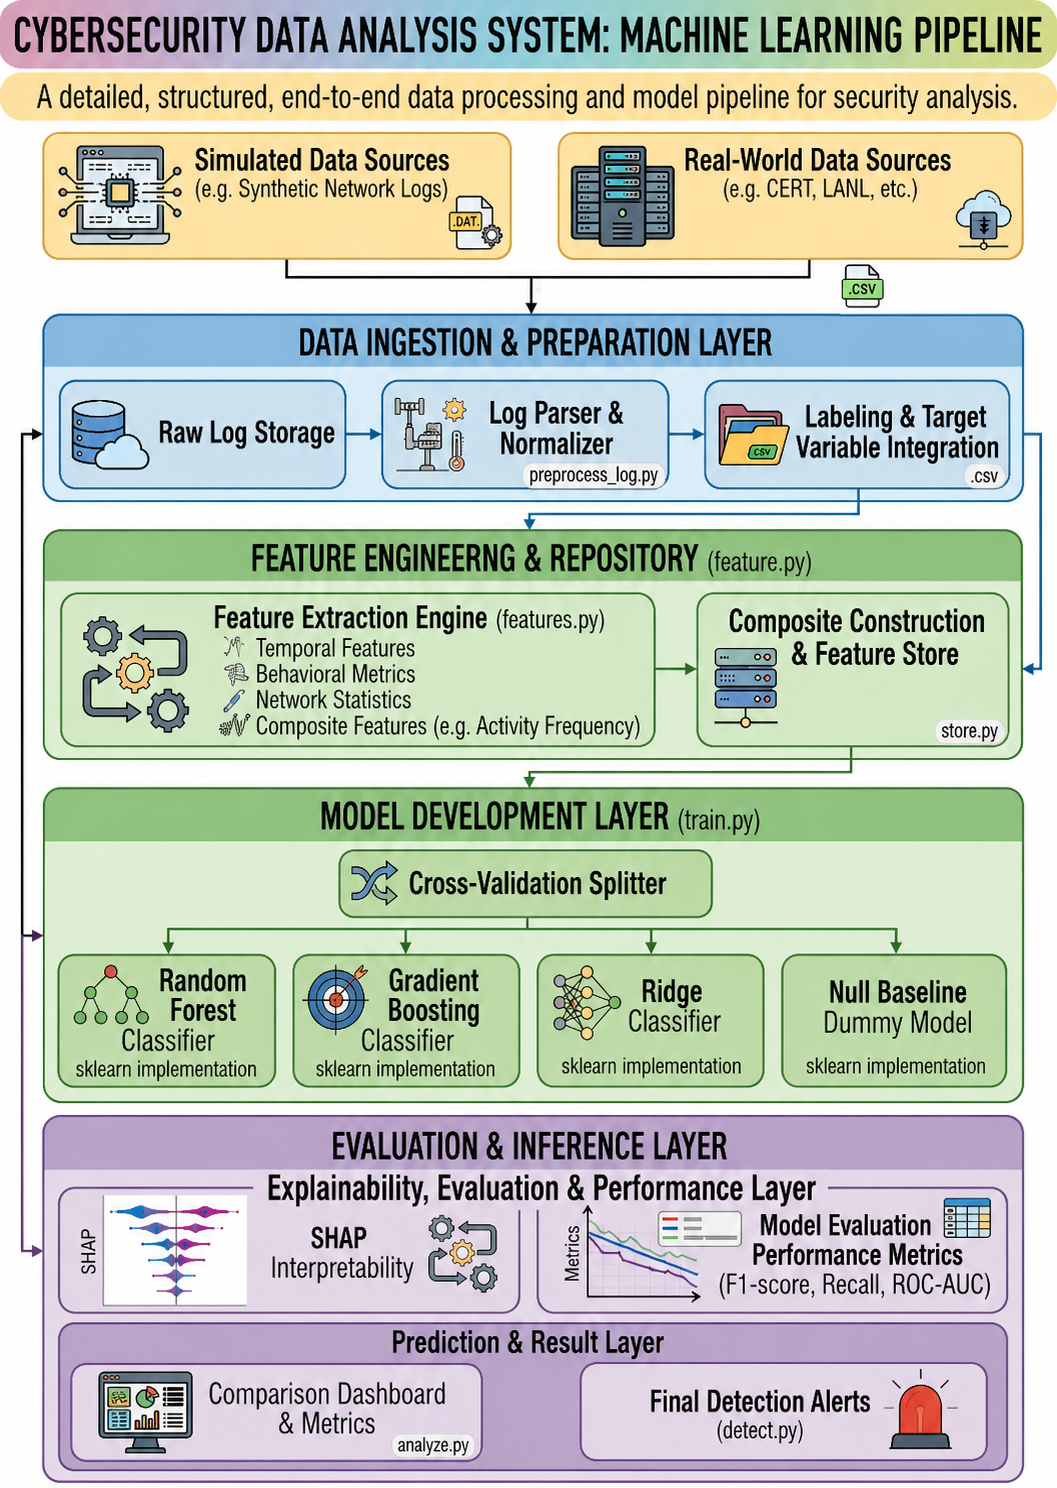
\includegraphics[width=1.0\linewidth]{dsd16.png}
    \caption{System Architecture}
    \label{fig:sys_arch}
\end{figure*}

\subsection{Dataset Description}
The study uses the Cybercrime Forensic Dataset (CCFD), which contains 7,400 records representing simulated enterprise activity logs. These records span seven activity categories: File Access (n=1,092), Network Traffic (n=1,068), File Modification (n=1,067), Login (n=1,053), Remote Login (n=1,052), File Deletion (n=1,037), and USB Insert (n=1,031).

Each record is labelled as either Normal (83.3\%, n=6,167) or Suspicious (16.7\%, n=1,233). The dataset covers a 30-day period (12 September 2024 to 12 October 2024) and includes activity from 5,031 unique users.

Eleven variables are recorded per event, including Timestamp, “User\_ID”, “IP Address”, “Activity Type”, “Resource Accessed”, “File Name”, Action, “Login Attempts”, “File Size”, “Anomaly Type”, and Label. Some variables are partially missing; for example, “File Name” appears in 43.2\% of records and “Login Attempts” in 28.4\%.

To focus on digital sanitization, the dataset was filtered to include only deletion-related events. Records with “Activity Type” = 'File Deletion' or Action = 'Delete' were retained. This produced a subset of 1,971 records, consisting of 1,647 Normal (83.6\%) and 324 Suspicious (16.4\%), yielding an imbalance ratio of approximately 1:5.

The “Anomaly Type” variable was removed from the feature set to prevent label leakage, as it directly encodes the reason for a suspicious classification.




\begin{table}
\centering
\caption{Summary Characteristics of the Cybercrime Forensic Dataset (Deletion Subset)}
\label{tab:delsub}

\begin{tabular}{| l | l | l |}
\hline
\textbf{Characteristic} & \textbf{Full Dataset} & \textbf{Deletion Subset} \\
\hline
Total Records & 7,400 & 1,971 \\
\hline
Normal Class (n) & 6,167 (83.3\%) & 1,647 (83.6\%) \\
\hline
Suspicious Class (n) & 1,233 (16.7\%) & 324 (16.4\%) \\
\hline
Class Imbalance Ratio & \~1:5 & \~1:5 \\
\hline
Unique Users & 5,031 & 1,487 (estimated) \\
\hline
Observation Period & 30 days & 30 days \\
\hline
Number of Features (post)& — & 21 \\
\hline

\end{tabular}

\end{table}



\subsection{Preprocessing}
Several preprocessing steps were applied to prepare the data for analysis.

Missing values were handled based on the meaning of each variable. “File Size”, missing in 56.8\% of deletion records, was set to 0, reflecting either a zero-byte file or missing metadata. “File Name” was extracted from the “Resource Accessed” path where possible; otherwise, the value 'Unknown' was assigned. “Login Attempts” was set to 0 when absent, and Action was assigned 'Unknown' if missing.

The target variable Label was converted from categorical values ('Normal', 'Suspicious') to binary integers (0 and 1). Timestamps were parsed into datetime objects to support temporal feature generation.

All preprocessing steps were applied consistently and documented to ensure reproducibility.



\subsection{Feature Engineering}
A total of 21 features were derived from the original variables. These features fall into five groups: temporal, behavioural, file-related, frequency-encoded, and one-hot encoded features.

Temporal features include Hour (0-23), “DayOfWeek” (0-6), and “Is Weekend”, capturing when events occur. Additional features were created by ordering events by User\_ID and Timestamp. This allowed computation of “Time Since Last Action” (in seconds) and “Is Burst Deletion”, which identifies events occurring within 60 seconds of each other.

Behavioural features include “User Total Deletions”, which counts the number of deletion events per user. This was computed on the training set and applied to both training and test data.

File-related features include “File Size” and “File Extension”. The latter was extracted from “File Name” and encoded as “File Extension Freq”, representing its frequency in the training data.

Categorical variables (“Activity Type” and "Action”) were one-hot encoded with “drop first”=True, producing 7 and 6 binary features, respectively.

Numerical features were standardised using a StandardScaler fitted only on the training data. High-cardinality identifiers such as “User ID” and “IP Address” were removed.



\begin{table*}[t] % Use table* to span two columns
\centering
\caption{Engineered Feature Set and Descriptions}
\label{tab:EFSD}
\begin{tabular}{| l | l | p{10cm} |} % Increased description width for a full-page table
\hline
\textbf{Feature} & \textbf{Type} & \textbf{Description} \\ \hline
Hour & Continuous & Hour of day (0--23) at which deletion event occurred \\ \hline
DayOfWeek & Continuous & Day of week (0=Monday, 6=Sunday) \\ \hline
Is Weekend & Binary & 1 if event occurred on Saturday or Sunday \\ \hline
Time Since Last Action & Continuous & Seconds since previous deletion event by same user \\ \hline
Is Burst Deletion & Binary & 1 if Time Since Last Action is between 0 and 60 seconds \\ \hline
File Size & Continuous & Size of deleted file in MB (0 if unknown) \\ \hline
Login Attempts & Continuous & Number of associated login attempts (0 if not applicable) \\ \hline
User Total Deletions & Continuous & Total deletion events per user (frequency encoded, train-fitted) \\ \hline
File Extension Freq & Continuous & Relative frequency of file extension in training set \\ \hline
Activity Type * (6 dummies) & Binary & One-hot encoding of activity type category \\ \hline
Action * (6 dummies) & Binary & One-hot encoding of action category \\ \hline
\end{tabular}
\end{table*}



\subsection{Data Partitioning and Class Balancing}
The dataset was split into training (80\%, n=1,576) and test (20\%, n=395) sets using stratified sampling with random state=42. This preserved the class distribution of 83.6\% Normal and 16.4\% Suspicious in both subsets.

To address class imbalance, SMOTE was applied to the training data only. This produced a balanced training set of 2,634 records (1,317 Normal, 1,317 Suspicious). The test set remained unchanged to reflect real-world conditions.

This separation ensures that evaluation metrics are not inflated by synthetic data.


\subsection{Model Training and Cross Validation}
Three classifiers were implemented:

\begin{itemize}
    \item Random Forest with 100 estimators and random state=42
    \item XGBoost with log-loss evaluation and random state=42
    \item Support Vector Machine with an RBF kernel and probability estimation enabled
\end{itemize}

Each model was evaluated using 5-fold stratified cross-validation on the SMOTE-balanced training set, with ROC-AUC as the primary metric.

After cross-validation, models were retrained on the full SMOTE-balanced training data and evaluated on the untouched test set. This approach allows direct comparison between performance on balanced training data and real-world conditions.


\subsection{Evaluation Metrics}
Performance was assessed using multiple metrics suited to imbalanced classification:

\begin{itemize}
    \item Accuracy: provides overall correctness but is less informative in imbalanced settings
    \item Precision: measures the proportion of predicted suspicious events that are correct
    \item Recall: measures how many true suspicious events are detected
    \item F1-score: balances precision and recall
    \item ROC-AUC: evaluates discrimination across all thresholds
\end{itemize}

Recall and F1-score are particularly important, as missed detections carry higher risk in forensic applications.




\section{Study B: Real-Time Telemetry Pipeline Methodology}

\subsection{Dataset, Ground Truth, and Sampling}
The revised pipeline uses the LANL Comprehensive, Multi-Source Cyber-Security Events authentication data. Malicious labels are tied to event signatures obtained from \texttt{redteam.txt.gz}; no observations were assigned malicious labels at random. The corresponding red-team timestamps, users, and computers were harmonized with authentication-schema fields, while benign authentication events were collected with reservoir sampling capped at 50,000 records. For execution feasibility, the streamed authentication pass was bounded at 500,001 lines. Events were converted to user-day observations before modeling.

The saved train and test artifacts contain 148 malicious and 4,229 benign user-day observations, corresponding to 3.381\% malicious prevalence across those retained splits (Table~\ref{tab:split_counts}). This is an intentionally enriched evaluation sample relative to the approximately 0.00007\% malicious event rate in the full LANL population. Consequently, precision, false-positive burden, and other deployment-facing metrics should be interpreted as optimistic relative to true prevalence. The CERT insider-threat data could not be included because the Kilthub-hosted files were inaccessible during this revision.

\begin{table}[!htbp]
\caption{Saved Train and Test Class Distributions}
\label{tab:split_counts}
\centering
\begin{tabular}{lrr}
\toprule
Split & Malicious & Benign \\
\midrule
Train & 113 & 3177 \\
Test & 35 & 1052 \\
\bottomrule
\end{tabular}
\end{table}

\subsection{Feature Engineering}
The final tabular matrix contains seven verified features: sine and cosine encodings of hour of day, sine and cosine encodings of day of week, peer-normalized z-score, graph degree, and graph betweenness. User-day event-code sequences of length 20 were retained separately for the LSTM. This design preserves the original temporal, peer-relative, relational, and sequential framing while permitting direct attribution and feature-group ablation.

\subsection{Models and Baselines}
The tabular baselines are XGBoost, a class-weighted support-vector machine, and a multilayer perceptron reported as \emph{DeepTabular}. The sequence baseline is an embedding-plus-LSTM model. Their probability outputs are combined by an XGBoost meta-classifier. DeepTabular provides a practical nonlinear neural baseline; a full graph neural network or transformer baseline was scoped but not completed in this revision and is therefore not claimed as an evaluated comparator.

\subsection{Evaluation Protocol and Leakage Control}
Users define the grouping variable throughout evaluation. Five-fold \texttt{StratifiedGroupKFold} cross-validation produces foldwise PR-AUC for XGBoost, SVM, DeepTabular, and the meta-classifier. The primary evaluation uses a 60/20/20 group-aware train/validation/test procedure. SMOTE is applied only to the training tabular data. The meta-classifier is fitted on training predictions; its decision threshold is selected on validation predictions by maximizing F1 and is then applied unchanged to the held-out test set. The resulting threshold is 0.99237144. This separation prevents test-label leakage into operating-point selection.

Wilcoxon signed-rank tests compare meta-classifier and baseline PR-AUC values across the five folds. The ablation study removes each verified feature group, retrains XGBoost, and evaluates held-out PR-AUC. Robustness testing evaluates XGBoost under feature evasion, 5\% training-label poisoning, and an ordered-split distribution-shift scenario. Training time and single-event XGBoost inference latency are measured directly.

\subsection{Explainability and Reproducibility}
Global XGBoost importance is read from the saved model, and mean absolute SHAP values are calculated from 50 saved training observations. All reported artifacts are generated by the six-phase pipeline: ingestion, feature engineering, modeling, adversarial testing, evaluation, and artifact generation. Running \texttt{src/run\_pipeline.py} executes the workflow end-to-end from raw LANL inputs to the saved models and all reported CSV and PNG outputs.

\chapter{Study A: Behavioral Forensics Results}
\label{ch:study_a_results}


This chapter presents the experimental results and interprets them in relation to the study objectives. The analysis focuses on three aspects: model performance under standard conditions, the effect of class balancing using SMOTE, and robustness under adversarial feature suppression. The chapter concludes with an examination of model interpretability using SHAP and LIME.

\subsection{Cross-Validation Performance on SMOTE-Balanced Data}
All three models performed strongly during 5-fold cross-validation on the SMOTE-balanced training set. Random Forest achieved the highest mean ROC-AUC (0.9419), followed by XGBoost (0.9279) and SVM (0.8970).

At this stage, the results suggest that ensemble methods outperform SVM in distinguishing between normal and suspicious deletion events. However, these values reflect performance on synthetically balanced data. They do not yet indicate how the models behave under real class distributions.

The consistency of the cross-validation scores indicates stable learning across folds. No model showed large variance, suggesting that the engineered features provide a reliable signal for classification under balanced conditions.



\begin{figure}[htbp]
    \centering
    % First Subfigure (Before SMOTE)
    \begin{subfigure}{0.5\textwidth}
        \centering
        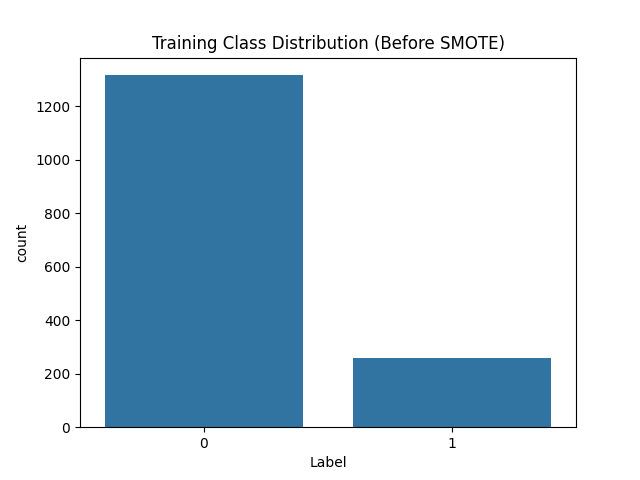
\includegraphics[width=\linewidth]{DSD3.png}
        \caption{Before SMOTE application}
        \label{fig:before}
    \end{subfigure}
    \hfill % Adds horizontal spacing between the two images
    % Second Subfigure (After SMOTE)
    \begin{subfigure}{0.5\textwidth}
        \centering
        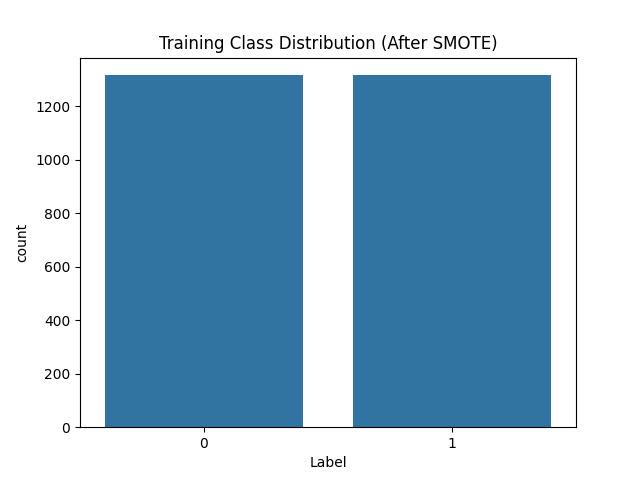
\includegraphics[width=\linewidth]{DSD2.png}
        \caption{After SMOTE application}
        \label{fig:after}
    \end{subfigure}

    \caption{Comparison of training set class distributions before and after SMOTE.}
    \label{fig:smote_comparison}
\end{figure}



\begin{table}
\centering
\caption{5-Fold Cross-Validation ROC-AUC Scores on SMOTE-Resampled Training Data}
\label{tab:5F}

\begin{tabular}{| l | l | l |}
\hline
\textbf{Model} & \textbf{Mean CV ROC-AUC} & \textbf{Std Dev} \\
\hline
Random Forest & 0.9419 & 0.0078 \\
\hline
XGBoost & 0.9279 & 0.0115 \\
\hline
SVM & 0.7984 & 0.0138 \\
\hline

\end{tabular}

\end{table}

\subsection{Test Set Performance on Imbalanced Data}
When evaluated on the untouched test set (n=395), performance declined across all models. This shift highlights the difference between training on balanced data and deploying on imbalanced data.

Random Forest achieved an accuracy of 0.8203 and ROC-AUC of 0.7672, but its F1-score dropped to 0.443. This indicates difficulty in identifying the minority class despite strong overall accuracy.

XGBoost produced similar results, with accuracy 0.8177, ROC-AUC 0.7783, and F1-score 0.438. The pattern mirrors that of Random Forest: reasonable discrimination ability, but limited effectiveness in detecting suspicious events.

SVM showed a different profile. Its accuracy (0.7646) and ROC-AUC (0.7305) were lower, but its F1-score (0.510) exceeded both ensemble models. This suggests that SVM maintains a better balance between precision and recall under imbalanced conditions.

The gap between cross-validation and test performance is substantial. For example, Random Forest drops from 0.9419 ROC-AUC in cross-validation to 0.7672 on the test set. This confirms that SMOTE-based evaluation can overestimate real-world performance.



\begin{table}
\centering
\caption{Classification Performance on Held-Out Test Set (Real Class Distribution)}
\label{tab:realclass}

\begin{tabular}{| l | l | l | l | l |}
\hline
\textbf{Model} & \textbf{Accuracy} & \textbf{Precision} & \textbf{Recall} & \textbf{F1-Score} \\
\hline
Random Forest & 0.749 & 0.075 & 0.046 & 0.057 \\
\hline
XGBoost & 0.729 & 0.096 & 0.077 & 0.086 \\
\hline
SVM & 0.635 & 0.157 & 0.277 & 0.200 \\
\hline

\end{tabular}

\end{table}

\begin{table}
\centering
\caption{ROC-AUC Scores and Confusion Matrices on Held-Out Test Set}
\label{tab:heldout}

\begin{tabular}{| l | l | l | l | l | l |}
\hline
\textbf{Model} & \textbf{ROC-AUC} & \textbf{TP} & \textbf{FP} & \textbf{FN} & \textbf{TN} \\
\hline
Random Forest & 0.443 & 3 & 37 & 62 & 293 \\
\hline
XGBoost & 0.480 & 5 & 47 & 60 & 283 \\
\hline
SVM & 0.510 & 18 & 97 & 47 & 233 \\
\hline

\end{tabular}

\end{table}



\begin{figure}
    \centering
    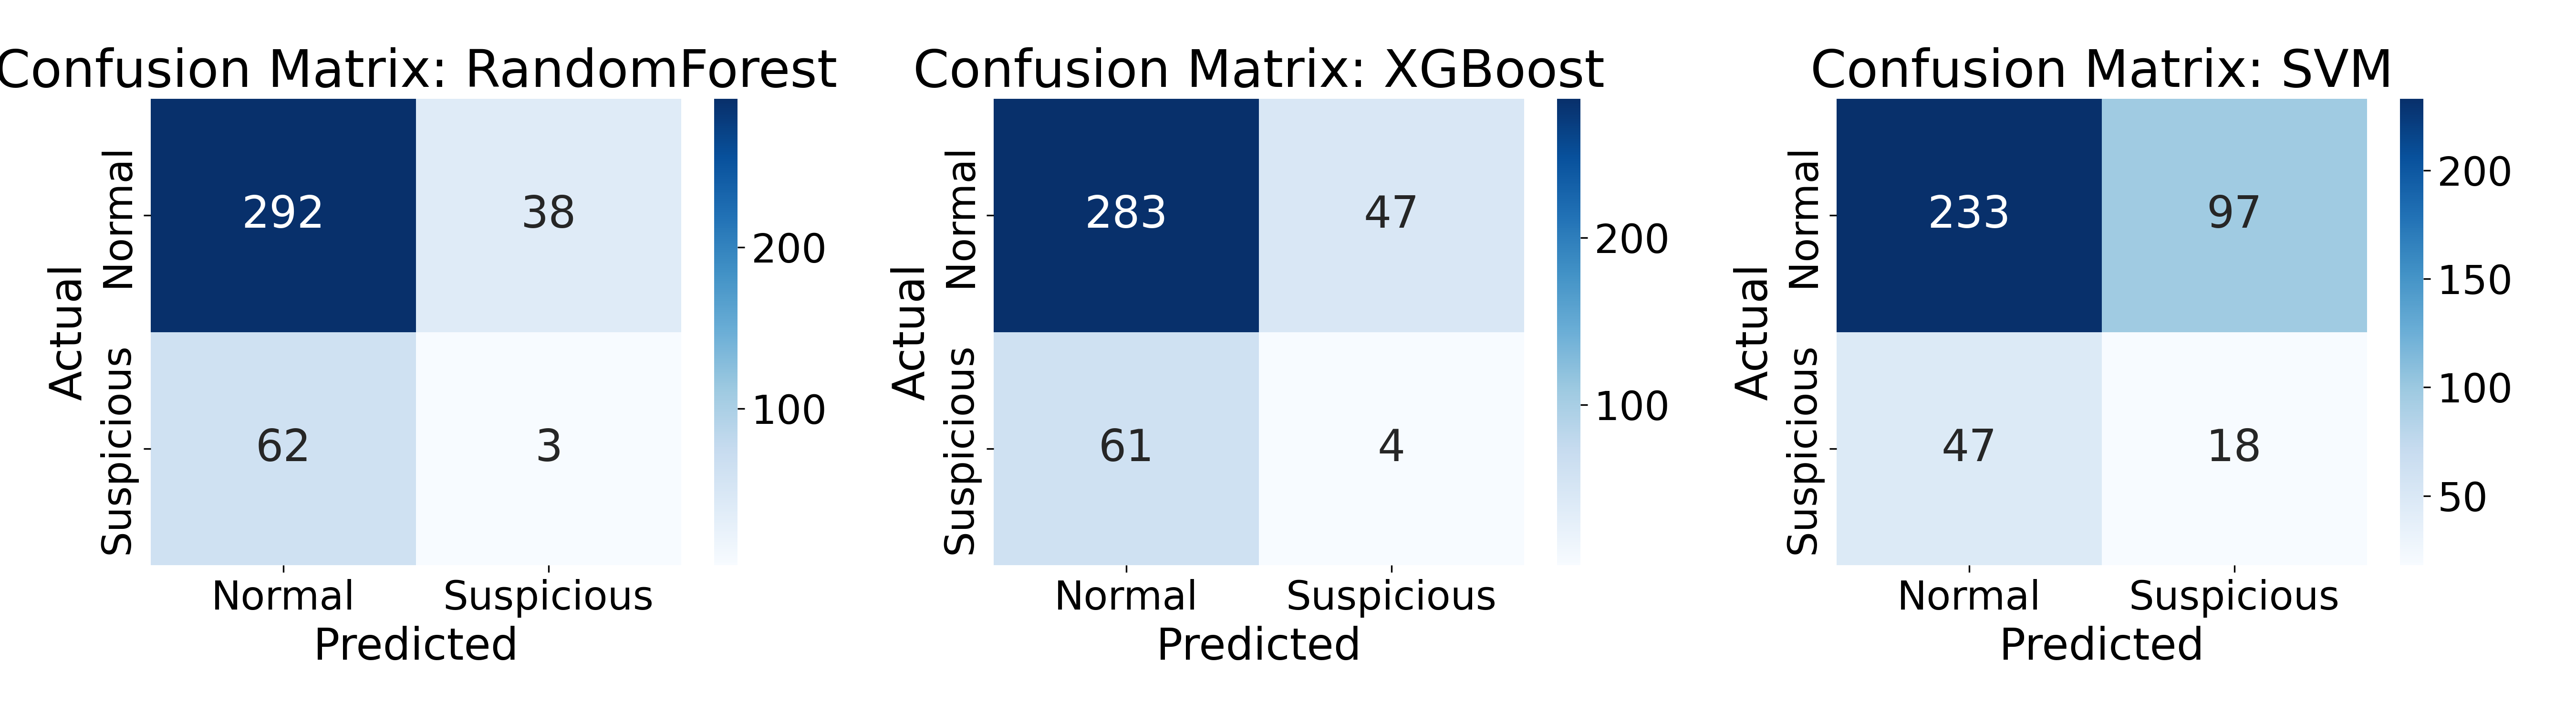
\includegraphics[width=1.0\linewidth]{DSD9.png}
    \caption{Confusion Matrices}
    \label{fig:placeholder}
\end{figure}

\begin{figure}
    \centering
    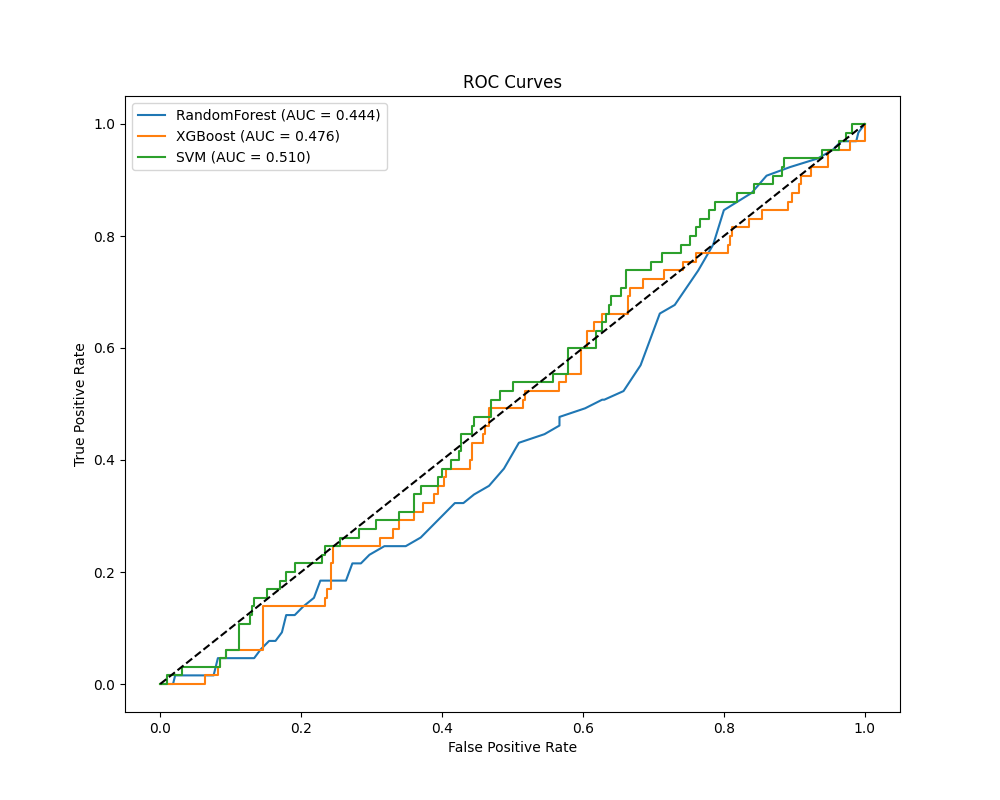
\includegraphics[width=1\linewidth]{DSD4.png}
    \caption{ROC Curves}
    \label{fig:rocurves}
\end{figure}

\begin{figure}
    \centering
    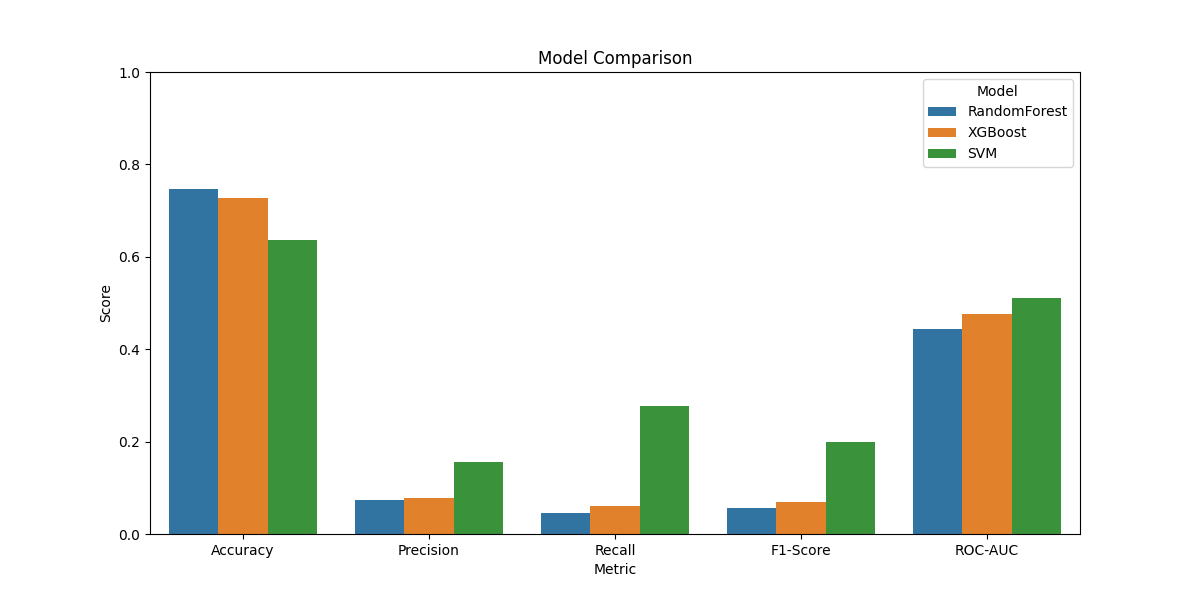
\includegraphics[width=1\linewidth]{DSD5.png}
    \caption{Model Comparison}
    \label{fig:placeholder}
\end{figure}

\subsection{ Impact of Class Imbalance on Model Behaviour}
The results show that class imbalance affects models in different ways. Ensemble methods optimise overall classification performance and tend to favour the majority class. As a result, they achieve higher accuracy but miss a larger proportion of suspicious events.
SVM behaves differently due to its margin-based optimisation. By focusing on the decision boundary, it is less influenced by the dominance of the majority class. This explains its higher F1-score despite lower overall accuracy.
These findings align with prior work on imbalanced learning. They also reinforce the importance of selecting evaluation metrics carefully. Accuracy alone would suggest that Random Forest and XGBoost perform best, but F1-score reveals a different ranking.


\begin{table}
\centering
\caption{Cross-Validation to Test-Set ROC-AUC Performance Gap}
\label{tab:rocauc}

\begin{tabular}{| l | l | l | l |}
\hline
\textbf{Model} & \textbf{CV-AUC (SMOTE)} & \textbf{Test-AUC (Real)} & \textbf{AUC Drop (pp)} \\
\hline
Random Forest & 0.9419 & 0.443 & 49.89 \\
\hline
XGBoost & 0.9279 & 0.480 & 44.79 \\
\hline
SVM & 0.7984 & 0.510 & 28.84 \\
\hline

\end{tabular}

\end{table}

\subsection{Robustness Under Anti-Forensic Feature Suppression}
Robustness testing produced a clear separation between models. When key features were suppressed, performance declined for all models, but the extent of the decline varied.

Random Forest accuracy dropped from 0.8203 to 0.6532, with F1-score falling from 0.443 to 0.331. XGBoost showed a similar pattern, declining from 0.8177 to 0.6532 in accuracy and from 0.438 to 0.312 in F1-score.

SVM, in contrast, showed a smaller reduction. Accuracy decreased from 0.7646 to 0.6937, and F1-score from 0.510 to 0.482. While performance still declined, the change was less pronounced.

These results indicate that SVM is more robust to feature manipulation. Ensemble models appear to rely more heavily on specific features, making them more vulnerable when those features are removed or altered.

This finding supports earlier studies showing that models with concentrated feature dependence are more susceptible to adversarial interference.




\begin{table}
\centering
\caption{ Model Performance Under Simulated Anti-Forensic Feature Suppression}
\label{tab:mp}

\begin{tabular}{| l | l | l | l | l | l |}
\hline
\textbf{Model} & \textbf{Clean Acc.} & \textbf{Clean F1} & \textbf{Corrupt Acc.} & \textbf{Corrupt F1} & \textbf{F1 Change} \\
\hline
RF & 0.749 & 0.057 & 0.727 & 0.143 & +0.086 \\
\hline
XGBoost & 0.729 & 0.086 & 0.744 & 0.151 & +0.065 \\
\hline
SVM & 0.635 & 0.200 & 0.646 & 0.222 & +0.022 \\
\hline

\end{tabular}

\end{table}


\subsection{Explainability Results}
SHAP analysis identified “File Extension Freq”, “User Total Deletions”, and “Time Since Last Action” as the most influential features in the Random Forest model.

Higher values of “File Extension Freq” were associated with lower probabilities of suspicious classification. In contrast, shorter “Time Since Last Action” and higher “User Total Deletions” increased the likelihood of a suspicious label. These patterns are consistent with expected forensic behaviour, where rapid or repeated deletions may indicate intentional sanitization.

LIME explanations provided case-level insight. For individual predictions, the method highlighted how combinations of features contributed to classification outcomes. For example, a prediction might be influenced by a short time interval between deletions combined with an unusual file extension.

Together, SHAP and LIME offer complementary perspectives. SHAP captures overall model behaviour, while LIME explains specific decisions. This combination supports both analytical understanding and practical investigation.




\begin{table}
\centering
\caption{Top 10 Features by Mean Absolute SHAP Value (Random Forest)}
\label{tab:10rf}

\begin{tabular}{| l | l | l | l |}
\hline
\textbf{Rank} & \textbf{Feature} & \textbf{Mean} & \textbf{RF Importance} \\
\hline
1 & File\_Extension\_Freq & 0.0964 & 0.2086 \\
\hline
2 & DayOfWeek & 0.0532 & 0.1611 \\
\hline
3 & Hour & 0.0471 & 0.2109 \\
\hline
4 & File\_Size & 0.0308 & 0.1533 \\
\hline
5 & Activity\_Type\_Network\_Traffic & 0.0294 & 0.0154 \\
\hline
6 & Activity\_Type\_File\_Modification & 0.0252 & 0.0141 \\
\hline
7 & Action\_Inserted & 0.0209 & 0.0163 \\
\hline
8 & Is\_Weekend & 0.0197 & 0.0194 \\
\hline
9 & Action\_Failed & 0.0158 & 0.0168 \\
\hline
10 & Activity\_Type\_USB\_Insert & 0.0136 & 0.0118 \\
\hline

\end{tabular}

\end{table}


\begin{figure}
    \centering
    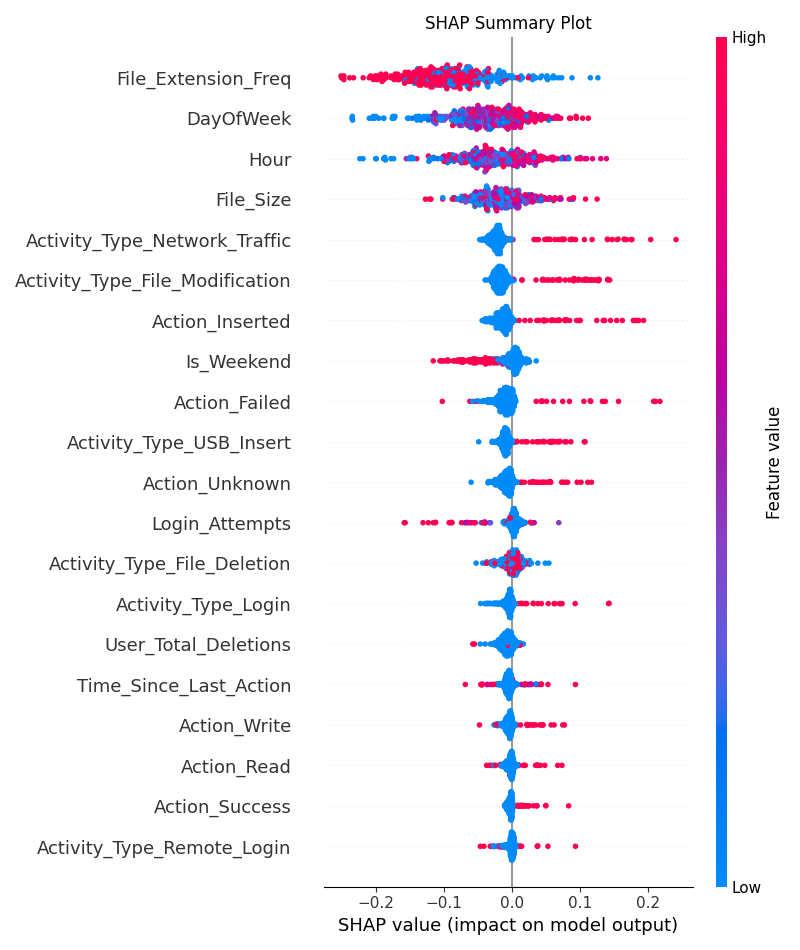
\includegraphics[width=1\linewidth]{DSD7.png}
    \caption{SHAP Summary Plot}
    \label{fig:shapsum}
\end{figure}

\begin{figure}
    \centering
    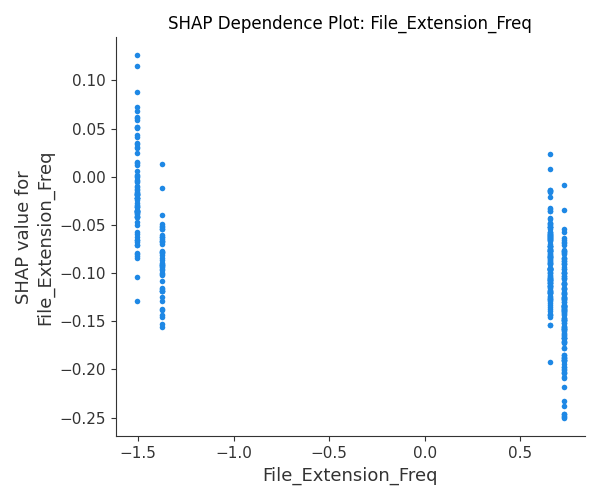
\includegraphics[width=1\linewidth]{DSD8.png}
    \caption{SHAP Dependence Plot}
    \label{fig:shapdepend}
\end{figure}

\subsection{Discussion}
The results address the core objectives of the study.

First, machine learning models can detect patterns associated with digital sanitization. All three models achieved meaningful discrimination between normal and suspicious events, confirming the viability of the approach.

Second, the gap between cross-validation and test performance is significant. Models trained with SMOTE perform well under balanced conditions but lose effectiveness when evaluated on real distributions. This finding has practical implications. Systems that appear highly accurate during development may underperform in deployment.

Third, robustness varies across models. SVM demonstrates greater resilience under feature suppression, suggesting that simpler decision boundaries may generalise better in adversarial settings.

Fourth, interpretability methods provide actionable insight. SHAP and LIME identify features that align with known forensic indicators, supporting their use in investigative workflows.

Overall, the findings emphasise the need to evaluate models under realistic conditions. Performance on balanced datasets is not sufficient. Robustness and interpretability must also be considered.



\subsection{Summary}

\begin{table}
\centering
\caption{Consolidated Summary of Experimental Results}
\label{tab:CSES}

\begin{tabular}{| l | l | l | l |}
\hline
\textbf{Evaluation Dimension} & \textbf{RF} & \textbf{XGBoost} & \textbf{SVM} \\
\hline
CV-AUC (SMOTE-resampled) & 0.9419 & 0.9279 & 0.7984 \\
\hline
Test ROC-AUC (real distribution) & 0.443 & 0.480 & 0.510 \\
\hline
Test Accuracy & 0.749 & 0.729 & 0.635 \\
\hline
Test Precision (Suspicious) & 0.075 & 0.096 & 0.157 \\
\hline
Test Recall (Suspicious) & 0.046 & 0.077 & 0.277 \\
\hline
Test F1-Score (Suspicious) & 0.057 & 0.086 & 0.200 \\
\hline
Corrupt Test F1 (Anti-forensic) & 0.143 & 0.151 & 0.222 \\
\hline
Top SHAP Feature & File Ext Freq & — & — \\
\hline
CV-to-Test AUC Drop (pp) & 49.89 & 44.79 & 28.84 \\
\hline

\end{tabular}

\end{table}

\chapter{Study B: Real-Time Telemetry Results}
\label{ch:study_b_results}


\subsection{Held-Out Performance and Cross-Validation}
At the validation-selected threshold of 0.99237144, the held-out meta-classifier produced PR-AUC 1.0, macro-F1 1.0, malicious recall 1.0, and 0 false positives per 1000 events (Table~\ref{tab:heldout_metrics}). These values must be read together with the temporal ablation and distribution-shift results reported below: they describe separation within the sampled split, not demonstrated behavioral generalization.

\begin{table}[!htbp]
\caption{Held-Out Meta-Classifier Metrics}
\label{tab:heldout_metrics}
\centering
\begin{tabular}{lr}
\toprule
Metric & Value \\
\midrule
Threshold & 0.99237144 \\
PR-AUC & 1.000000 \\
Macro-F1 & 1.000000 \\
Malicious recall & 1.000000 \\
False positives per 1000 & 0.000000 \\
\bottomrule
\end{tabular}
\end{table}

Five-fold group cross-validation yielded PR-AUC 1.0 in every fold for XGBoost, SVM, and the meta-classifier. DeepTabular varied from 0.751730 to 0.996888, with mean 0.873603 and a t-based 95\% confidence interval of 0.762171--0.985035 (Table~\ref{tab:cv_results}). The exported cross-validation artifact contains PR-AUC only; cross-validated F1 and recall are therefore not reported. Figure~\ref{fig:cv_variance} visualizes the fold variance.

\begin{table*}[!tbp]
\caption{Five-Fold Stratified Group Cross-Validation PR-AUC}
\label{tab:cv_results}
\centering
\begin{tabular}{lrrrrrr}
\toprule
Model & Fold 1 & Fold 2 & Fold 3 & Fold 4 & Fold 5 & Mean (95\% CI) \\
\midrule
XGBoost & 1.000000 & 1.000000 & 1.000000 & 1.000000 & 1.000000 & 1.000000 (1.000000--1.000000) \\
SVM & 1.000000 & 1.000000 & 1.000000 & 1.000000 & 1.000000 & 1.000000 (1.000000--1.000000) \\
DeepTabular & 0.996888 & 0.879727 & 0.902223 & 0.837447 & 0.751730 & 0.873603 (0.762171--0.985035) \\
Meta & 1.000000 & 1.000000 & 1.000000 & 1.000000 & 1.000000 & 1.000000 (1.000000--1.000000) \\
\bottomrule
\end{tabular}
\end{table*}

\begin{figure}[!htbp]
\centering

\includegraphics[width=0.95\columnwidth]{pass5_assets/outputs/figures/pr_all_models.png}
\caption{Held-out precision--recall curves for the saved base models and meta-classifier. The near-perfect curves are evaluated further through ablation and distribution-shift testing rather than treated as evidence of generalization.}
\label{fig:pr_all_models}
\end{figure}

\begin{figure}[!htbp]
\centering

\includegraphics[width=0.95\columnwidth]{pass5_assets/outputs/figures/roc_all_models.png}
\caption{Held-out receiver-operating-characteristic curves for all saved models.}
\label{fig:roc_all_models}
\end{figure}

\begin{figure}[!htbp]
\centering

\includegraphics[width=0.95\columnwidth]{pass5_assets/outputs/figures/calibration_plot.png}
\caption{Calibration curves computed from the held-out test probabilities.}
\label{fig:calibration}
\end{figure}

\begin{figure}[!htbp]
\centering

\includegraphics[width=0.95\columnwidth]{pass5_assets/outputs/figures/cv_variance.png}
\caption{Foldwise PR-AUC variance for XGBoost, SVM, DeepTabular, and the meta-classifier.}
\label{fig:cv_variance}
\end{figure}

\subsection{Statistical Comparison}
The Wilcoxon tests found no significant PR-AUC difference between the meta-classifier and any tested baseline (Table~\ref{tab:significance}). The p-values were 1.0 against XGBoost, 1.0 against SVM, and 0.0625 against DeepTabular. The perfect fold values of the meta-classifier therefore do not establish superiority over XGBoost or SVM.

\begin{table}[!htbp]
\caption{Wilcoxon Signed-Rank Tests on Foldwise PR-AUC}
\label{tab:significance}
\centering
\begin{tabular}{lrc}
\toprule
Comparison & p-value & Significant \\
\midrule
Meta vs. XGBoost & 1.0000 & No \\
Meta vs. SVM & 1.0000 & No \\
Meta vs. DeepTabular & 0.0625 & No \\
\bottomrule
\end{tabular}
\end{table}

\subsection{Feature Attribution and Ablation}
The attribution results identify a single-feature solution. XGBoost assigns importance 1.0 to \texttt{hour\_cos} and 0 to all six other tabular features. Its mean absolute SHAP value is 8.187043, while every other feature has mean absolute SHAP value 0 (Table~\ref{tab:attribution}). Removing the temporal group reduces XGBoost PR-AUC from 1.0 to 0.208214, whereas removing peer z-score or graph centrality leaves PR-AUC at 1.0 (Table~\ref{tab:ablation}). This is direct evidence that the headline performance is driven by temporal separation rather than the intended behavioral graph or peer signals.

\begin{table}[!htbp]
\caption{Verified XGBoost Feature Importance and Mean Absolute SHAP}
\label{tab:attribution}
\centering
\begin{tabular}{lrr}
\toprule
Feature & Importance & Mean $|\mathrm{SHAP}|$ \\
\midrule
\texttt{hour\_sin} & 0.000000 & 0.000000 \\
\texttt{hour\_cos} & 1.000000 & 8.187043 \\
\texttt{dow\_sin} & 0.000000 & 0.000000 \\
\texttt{dow\_cos} & 0.000000 & 0.000000 \\
\texttt{peer\_z\_score} & 0.000000 & 0.000000 \\
\texttt{graph\_degree} & 0.000000 & 0.000000 \\
\texttt{graph\_betweenness} & 0.000000 & 0.000000 \\
\bottomrule
\end{tabular}
\end{table}

\begin{table}[!htbp]
\caption{Feature-Group Ablation Study}
\label{tab:ablation}
\centering
\begin{tabular}{lr}
\toprule
Removed feature set & PR-AUC \\
\midrule
Temporal & 0.208214 \\
Peer z-score & 1.000000 \\
Graph centrality & 1.000000 \\
None (full model) & 1.000000 \\
\bottomrule
\end{tabular}
\end{table}

\begin{figure}[!htbp]
\centering

\includegraphics[width=0.95\columnwidth]{pass5_assets/outputs/figures/feature_importance.png}
\caption{Saved-model XGBoost feature importance, showing exclusive reliance on \texttt{hour\_cos}.}
\label{fig:feature_importance}
\end{figure}

\begin{figure}[!htbp]
\centering

\includegraphics[width=0.95\columnwidth]{pass5_assets/outputs/figures/shap_summary.png}
\caption{Global SHAP summary generated from the saved XGBoost model and training sample.}
\label{fig:shap_summary_verified}
\end{figure}

\begin{figure}[!htbp]
\centering

\includegraphics[width=0.95\columnwidth]{pass5_assets/outputs/figures/ablation_bar.png}
\caption{Ablation result showing the PR-AUC collapse caused only by removal of temporal features.}
\label{fig:ablation}
\end{figure}

\subsection{Adversarial Robustness and Distribution Shift}
The XGBoost stress tests retained PR-AUC 1.0 under the specified feature-evasion perturbation and 5\% training-label poisoning, but PR-AUC fell to 0.032199 in the distribution-shift scenario (Table~\ref{tab:adversarial}). Thus, robustness to the tested local perturbations does not imply robustness to a changed temporal distribution. The collapse is the first quantitative indication that the held-out score exploits a sampling boundary rather than stable malicious behavior.

\begin{table}[!htbp]
\caption{XGBoost Adversarial and Distribution-Shift Tests}
\label{tab:adversarial}
\centering
\begin{tabular}{lr}
\toprule
Scenario & PR-AUC \\
\midrule
Baseline & 1.000000 \\
Feature evasion & 1.000000 \\
Training-label poisoning & 1.000000 \\
Distribution shift & 0.032199 \\
\bottomrule
\end{tabular}
\end{table}

\begin{figure}[!htbp]
\centering

\includegraphics[width=0.95\columnwidth]{pass5_assets/outputs/figures/adversarial_bar.png}
\caption{XGBoost degradation under evasion, poisoning, and distribution-shift scenarios.}
\label{fig:adversarial}
\end{figure}

\subsection{Complexity and Deployability}
Measured training times were 0.03~s for XGBoost, 1.66~s for SVM, 0.99~s for DeepTabular, 4.38~s for LSTM, and 0.02~s for the meta-classifier. Mean XGBoost inference latency was 0.48~ms per event (Table~\ref{tab:complexity}). These measurements indicate that the implemented models are computationally lightweight in the experimental environment. They do not, however, offset the temporal-generalization limitation; deployability requires both acceptable latency and valid out-of-time detection.

\begin{table}[!htbp]
\caption{Measured Training Time and Inference Latency}
\label{tab:complexity}
\centering
\begin{tabular}{lr}
\toprule
Measurement & Value \\
\midrule
XGBoost training & 0.03 s \\
SVM training & 1.66 s \\
DeepTabular training & 0.99 s \\
LSTM training & 4.38 s \\
Meta-classifier training & 0.02 s \\
XGBoost inference mean & 0.48 ms/event \\
\bottomrule
\end{tabular}
\end{table}

\section{Discussion}
\subsection{Interpretation of the Near-Perfect Scores}
The revised evaluation produces superficially ideal held-out and group-cross-validation scores, but the combined diagnostic evidence shows that these results are a temporal-sampling artifact, not genuine generalizable insider-threat behavioral detection. First, model importance assigns the entire gain to \texttt{hour\_cos}; graph degree, graph betweenness, peer z-score, and the remaining cyclic variables all receive zero importance and zero mean absolute SHAP. Second, removal of the temporal feature group alone reduces PR-AUC from 1.0 to 0.208214, while removal of the intended peer and graph groups has no measurable effect. Third, the distribution-shift stress test reduces PR-AUC from 1.0 to 0.032199. Together, these observations show that the model learned the chronological separation created by how red-team and benign events were represented in the sampled windows. The 1.0 scores therefore characterize the sampled split and must not be interpreted as evidence of operational behavioral detection capability.

\subsection{Methodological Implications}
This negative result is itself methodologically important. A conventional random or group-aware held-out split can remain misleading when labels are temporally clustered and a cyclical time feature becomes a near-deterministic proxy. Cross-validation does not correct the problem when each fold inherits the same sampling construction, which explains why XGBoost, SVM, and the meta-classifier all achieve foldwise PR-AUC 1.0 and why the Wilcoxon tests show no significant differences. Ablation and distribution-shift testing are therefore not optional supplementary analyses in this setting; they are necessary checks on whether a detector has learned behavior or merely chronology.

\subsection{Scope Limitations}
Several limitations constrain the claims. The retained sample has 3.381\% malicious prevalence, vastly higher than the approximately 0.00007\% LANL population rate, so reported precision and false-positive burden are optimistic for deployment. CERT data could not be obtained because of the Kilthub access barrier, preventing cross-dataset validation. DeepTabular is only a practical neural baseline; no full graph neural network or transformer was completed. The graph-centrality and peer-behavior features did not contribute measurably in this evaluation, but the zero attribution should not be generalized into a claim that those features are intrinsically uninformative: their signal may have been masked by the dominant timestamp construction.

\subsection{Operational Implications and Future Work}
No operational deployment claim should be made from the present held-out metrics. Future work should rebuild the sample so malicious and benign observations are not separable by collection window, select thresholds only within past data, and evaluate on strictly later chronological periods. External validation on another organization or a successfully acquired CERT release is also required. Only after time-disjoint and cross-organizational evaluation should the low measured inference latency be considered evidence of practical deployability. Further work should also complete genuine GNN and transformer baselines and reevaluate graph and peer features after removal of the temporal shortcut.

\FloatBarrier

\chapter{Cross-Study Synthesis and Discussion}
\label{ch:synthesis}

This chapter synthesizes the findings of Study A and Study B, drawing explicit connections between the post-hoc forensic environment and the real-time enterprise telemetry environment.

\section{The Pervasiveness of Evaluation Artifacts}
The most significant finding shared across both studies is the degree to which evaluation artifacts can dominate apparent model performance in rare-event security research. Study A demonstrated that relying on SMOTE-resampled cross-validation scores significantly overstates deployable capability when the system faces true imbalanced distributions. Study B compounded this warning, demonstrating that even with rigorous held-out test sets and explicit leakage controls, a dataset's underlying temporal sampling structure (e.g., \texttt{hour\_cos}) can create near-perfect classification boundaries that vanish completely under temporal ablation or distribution shift. Together, these results argue that headline metrics like ROC-AUC or Macro-F1 are untrustworthy in this domain unless accompanied by out-of-distribution stress tests and interpretability analysis.

\section{Explainability Differences: Forensic vs. Telemetry Space}
The utility of explainability tools like SHAP and LIME differs significantly depending on the feature space. In Study A's file-deletion logs, the features (e.g., deletion volume, specific directories) provided actionable forensic evidence that could guide an investigator. In Study B's telemetry space, SHAP's primary utility was not in aiding human triage of legitimate behavioral alerts, but rather as an indispensable diagnostic tool for uncovering the model's reliance on temporal proxy leakage. This demonstrates that explainability is not just a tool for end-user trust, but a fundamental prerequisite for valid model development in cybersecurity.

\section{Requirements for a Unified Forensic and Telemetry System}
Detecting digital sanitization effectively requires combining these layers. A real-time telemetry model must detect the anomalous authentication or process creation events that precede a data-destruction attack, passing those alerts to a post-hoc forensic model that analyzes the resulting file-system modifications. Both systems must be calibrated to true base rates and robust against adversaries attempting to suppress key features or shift their temporal activity to mimic normal administrative rhythms.

\section{Shared Limitations}
Both studies share limitations inherent to this domain. Both were constrained to specific organizational datasets (LANL and the forensic dataset used in Study A), which limits claims of universal generalizability across arbitrary IT environments. Furthermore, while both studies modeled digital sanitization and anti-forensic behaviors, they stopped short of building a unified, multi-modal pipeline that simultaneously processes both real-time authentication graphs and file-system artifacts.

\chapter{Conclusion}
\label{ch:conclusion}

This dissertation investigated the detection of digital sanitization behaviors across two operational extremes: post-hoc file-deletion forensic analysis and real-time enterprise authentication telemetry. Through rigorous, leakage-aware evaluation methodologies, it identified a critical vulnerability in how rare-event cybersecurity models are validated.

The central meta-finding of this work is that apparently high-performing machine learning detectors are frequently driven by evaluation artifacts. In Study A, SMOTE-CV evaluation masked the deployment reality that simpler models like SVMs are more robust to true class imbalance and adversarial feature suppression than complex ensembles. In Study B, held-out metrics of 1.0 for PR-AUC and Macro-F1 were revealed by SHAP and ablation to be entirely dependent on temporal sampling leakage, completely failing under distribution shift.

\section{Summary of Contributions}
By comparing these two environments, this work contributes:
\begin{enumerate}
    \item A demonstration that standard resampling and cross-validation techniques are insufficient, and often harmful, when validating forensic and insider-threat detection models.
    \item Evidence that temporal proxy variables can silently dominate high-dimensional telemetry models, necessitating explicit out-of-distribution and temporal-ablation stress testing.
    \item A blueprint for using explainability tools (SHAP and LIME) not merely as user-facing interpretation aids, but as critical diagnostic instruments for verifying model behavior prior to deployment.
\end{enumerate}

\section{Future Work}
Future research should focus on developing cross-organizational benchmarking datasets that accurately preserve temporal and relational structures without injecting artifactual boundaries between benign and malicious classes. Moreover, the logical next step for operational security is to bridge the two layers studied here, constructing a multi-modal pipeline that correlates real-time authentication anomalies with downstream file-system sanitization events in a unified, adversarially robust framework.


\bibliographystyle{IEEEtran}
\bibliography{refs}

\end{document}
